\subsection{Studio della geometria dell'apparato}
Si è voluto studiare se la sorgente è posta effettivamente al centro dell'asse di rotazione o meno. Per farlo si sono semplicemente presi dei dati per un tempo
costante al variare dell'angolo, e è confrontata la rate con cui tali dati sono stati raccolti. In questo modo si avrà una stima della distanza tra sorgente e
rivelatore al variare dell'angolo del rivelatore stesso. I risultati si possono vedere nella Tabella \ref{tab:asse_dati}, dove l'errore sulle rate è stato preso
come errore poissoniano sui conteggi e considerando che il tempo non ha errore.
%
\begin{table}[h]
	\centering
	\begin{center}
\begin{tabulary}{\textwidth}{CCC}
\toprule
Angolo [gradi]	& rate [kHz]	& Errore [kHz]	\\ \midrule
0		& 8.301		& 0.004		\\ \midrule
20		& 8.331		& 0.004		\\ \midrule
40		& 8.362		& 0.004		\\ \midrule
50		& 8.387		& 0.004		\\ \midrule
70		& 8.420		& 0.004		\\ \midrule
90		& 8.437		& 0.004		\\
\bottomrule
\end{tabulary}
\end{center}  

	\caption{Rate di acquisizione al variare dell'angolo del rivelatore.}
	\label{tab:asse_dati}
\end{table}
%
Per trovare ora la posizione dell'asse di rotazione rispetto a quella della sorgente si vada nel sistema di riferimento in cui l'origine è l'asse di rotazione stesso.
Considerando il rivelatore come di dimensione piccola rispetto alla sua distanza dalla sorgente, si ha che la frequenza con cui registra dati va come $1/r^2$, con $r$ distanza
tra rivelatore e sorgente. Si consideri un sistema di riferimento in modo tale che il rivelatore a 0$^\circ$ giaccia sul semiasse negativo delle ascisse, e l'asse di
rotazione sia sullo zero, e si riscali in maniera che il rivelatore giaccia nelle coordinate (-1,0). In questo modo la distanza tra rivelatore e sorgente sarà presa come 1,
e sarà la distanza di riferimento. Allora, nelle altre configurazioni, considerando la rotazione come perfetta (cioè rotazione attorno ad un asse realmente unidimensionale),
si ha che nelle altre configurazioni il rivelatore occupa delle coordinate nel sistema cartesiano facilmente ricavabili a partire da funzioni goniometriche, e la distanza
dalla sorgente si ottiene a partire da quella di riferimento moltiplicandola per un fattore $\sqrt{\frac{\nu_0}{\nu_\theta}}$, cioè per la radice del rapporto tra la rate
di riferimento e a quell'angolo. Per calcolare le grandezze allora si trova da ragionamenti di natura geometrica:
$$ x_\theta = x_0 \cos \theta \hspace{1.5cm} y_\theta = y_0 \sin \theta \hspace{1.5cm} r_\theta = r_0 \sqrt{\frac{\nu_\theta}{\nu_0}}$$
Per fare questi calcoli si è trascurato l'errore sulle rate (e quindi sulle distanze): dato che i conteggi non sono così differenti tra loro, l'errore si approssima con facilità
ad essere uguale per tutte le configurazioni, quindi è sufficiente minimizzare la distanza dai cerchi per trovare il valore più palusibile della posizione della sorgente.
I cerchi si possono vedere nella Figura \ref{fig:asse_rotazione}\\
\begin{tikzpicture}[scale=1.4, spy using outlines={ magnification=10, size=3cm, connect spies,every spy on node/.append style={ultra thin}}]
\draw[->,thick] (-2,0)--(2,0) node[right]{$x$};
\draw[->,thick] (0,-2)--(0,2) node[above]{$y$};

\draw(-1,0) circle(1);
\draw[red, line width=0.0mm]({-cos(20)},{sin(20)}) circle(0.998197872);
\draw[blue, line width=0.0mm]({-cos(40)},{sin(40)}) circle(0.9963458709);
\draw[green, line width=0.0mm]({-cos(50)},{sin(50)}) circle(0.994859807);
\draw[cyan, line width=0.0mm]({-cos(70)},{sin(70)}) circle(0.99485981);
\draw[magenta, line width=0.0mm]({-cos(90)},{sin(90)}) circle(0.991907519);


\node [label=below left:0,draw,fill=black,circle,inner sep=0pt,minimum size=3pt] at (-1,0) {};
\node [label=left:20,draw,fill=black,circle,inner sep=0pt,minimum size=3pt, red] at ({-cos(20)},{sin(20)}) {};
\node [label=left:40,draw,fill=black,circle,inner sep=0pt,minimum size=3pt, blue] at ({-cos(40)},{sin(40)}) {};
\node [label=above left:50,draw,fill=black,circle,inner sep=0pt,minimum size=3pt, green] at ({-cos(50)},{sin(50)}) {};
\node [label=above left:70,draw,fill=black,circle,inner sep=0pt,minimum size=3pt, cyan] at ({-cos(70)},{sin(70)}) {};
\node [label=above:90,draw,fill=black,circle,inner sep=0pt,minimum size=3pt, magenta] at ({-cos(90)},{sin(90)}) {};


%\usetikzlibrary{spy}
\spy on (0,0) in node [left] at (6.5,1);

%\draw(-1.5,-2)--(1.5,-2);
%\draw(0,-2) ellipse[x radius = 1.5,y radius = 1];

%\node [label=below right:-R/2,draw,fill=black,circle,inner sep=0pt,minimum size=3pt] at (0,-2) {};
%\draw[decorate, decoration={brace, mirror}] (-1.5,-2.1) -- (0,-2.1);
%\draw[decorate, decoration=brace] (-0.1,-2) -- (-0.1,-1);

%\node [label= left :$r \cos 30$] at (-0.11,-1.5) {};
%\node [label= below :$r$] at (-0.75,-2.11) {};
%\node [label= above right :$R$] at (4,0) {};

%\node [label=above right:C,draw,fill=black,circle,inner sep=0pt,minimum size=3pt] at (0,1) {};
%\node [label=below:F,draw,fill=black,circle,inner sep=0pt,minimum size=3pt] at (-0.87,0) {};
%\node [label=below:F',draw,fill=black,circle,inner sep=0pt,minimum size=3pt] at (0.87,0) {};
%\node [label=below left:-R/2,draw,fill=black,circle,inner sep=0pt,minimum size=3pt] at (-4,0) {};
\end{tikzpicture} 


Si consideri la funzione che descrive la distanza della
sorgente dal rivelatore. Si ha che la distanza tra un punto $(x,y)$ e il rivelatore nella posizione $\theta$ è data da
$$\sqrt{(x-x_\theta)^2+(y-y_\theta)^2} = \sqrt{(x+\cos(\theta))^2+(y-\sin(\theta))^2}$$
Perciò andando a vedere il raggio stimato precedentemente come valore atteso della distanza, si può fare un fit a due parametri liberi con sei punti per ottenere
l'effettiva posizione nel piano della sorgente rispetto all'asse di rotazione. Si esegue questa operazione, andando a trovare il grafico che si può vedere nella
Figura \ref{gr:asse_bidim_2}. Questo rivela come la sorgente sia nel punto:
$$(0.0007 \pm 0.0004, 0.0076 \pm 0.0004)$$
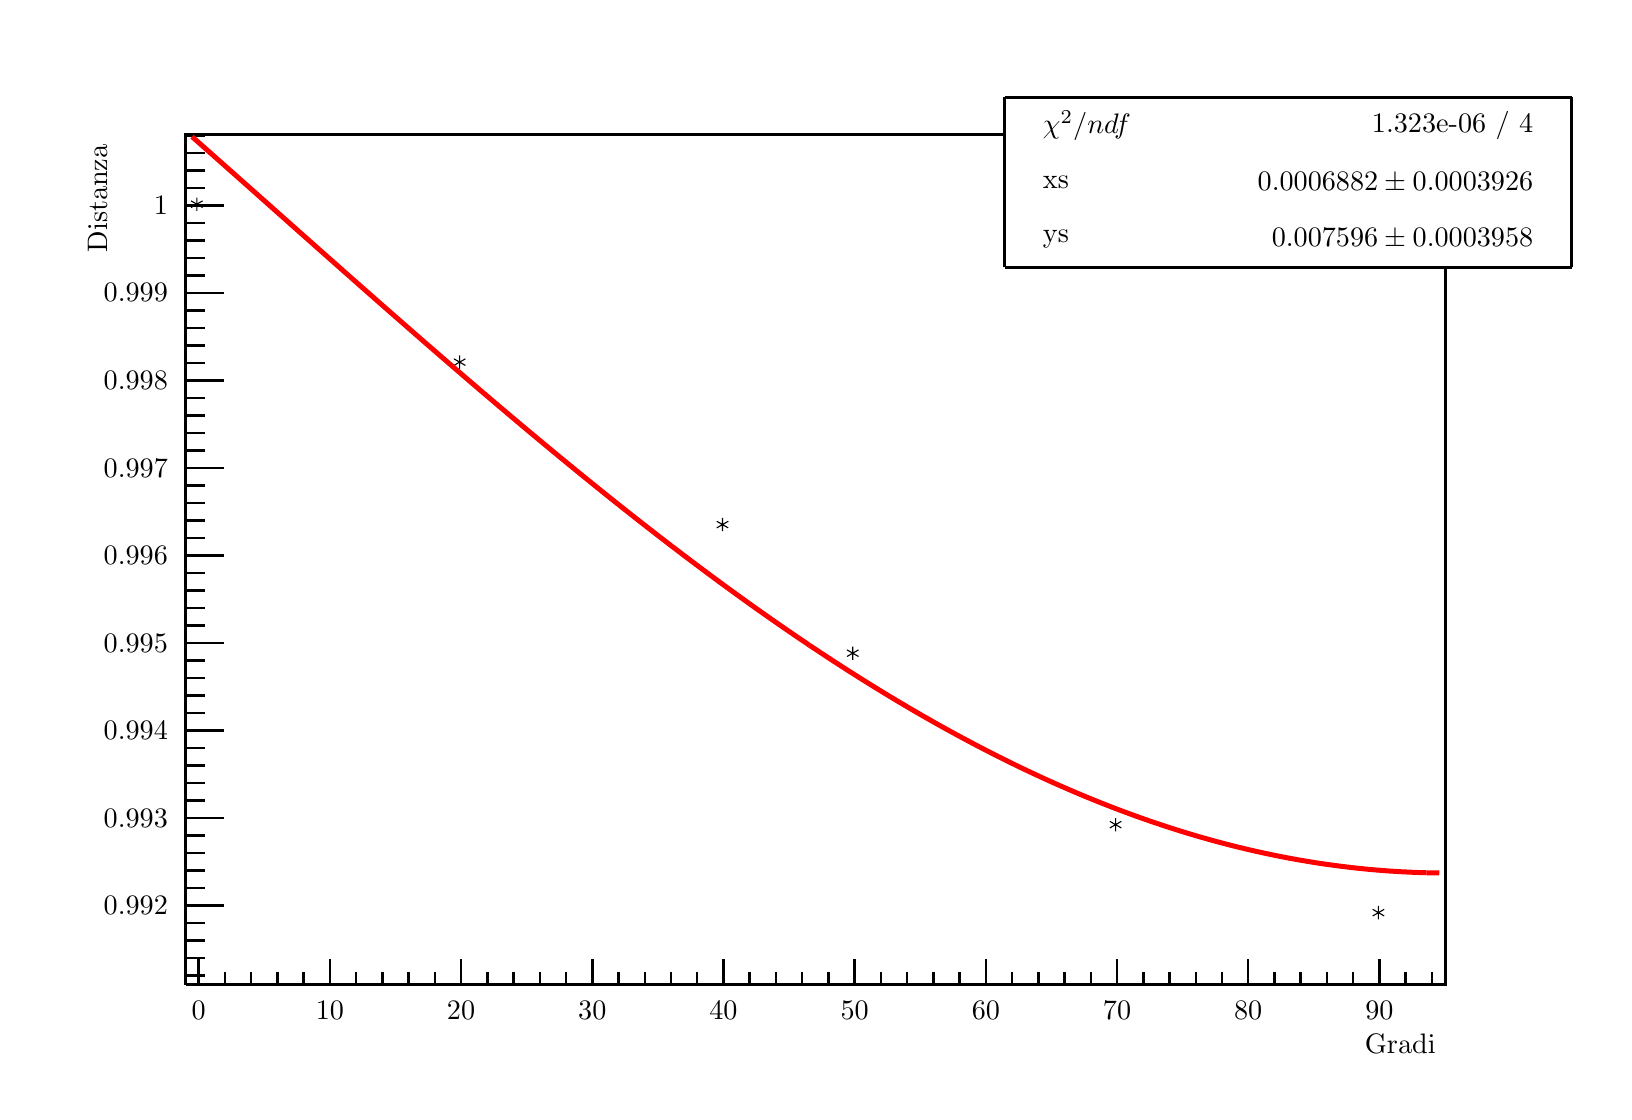
\begin{tikzpicture}
\pgfdeclareplotmark{cross} {
\pgfpathmoveto{\pgfpoint{-0.3\pgfplotmarksize}{\pgfplotmarksize}}
\pgfpathlineto{\pgfpoint{+0.3\pgfplotmarksize}{\pgfplotmarksize}}
\pgfpathlineto{\pgfpoint{+0.3\pgfplotmarksize}{0.3\pgfplotmarksize}}
\pgfpathlineto{\pgfpoint{+1\pgfplotmarksize}{0.3\pgfplotmarksize}}
\pgfpathlineto{\pgfpoint{+1\pgfplotmarksize}{-0.3\pgfplotmarksize}}
\pgfpathlineto{\pgfpoint{+0.3\pgfplotmarksize}{-0.3\pgfplotmarksize}}
\pgfpathlineto{\pgfpoint{+0.3\pgfplotmarksize}{-1.\pgfplotmarksize}}
\pgfpathlineto{\pgfpoint{-0.3\pgfplotmarksize}{-1.\pgfplotmarksize}}
\pgfpathlineto{\pgfpoint{-0.3\pgfplotmarksize}{-0.3\pgfplotmarksize}}
\pgfpathlineto{\pgfpoint{-1.\pgfplotmarksize}{-0.3\pgfplotmarksize}}
\pgfpathlineto{\pgfpoint{-1.\pgfplotmarksize}{0.3\pgfplotmarksize}}
\pgfpathlineto{\pgfpoint{-0.3\pgfplotmarksize}{0.3\pgfplotmarksize}}
\pgfpathclose
\pgfusepathqstroke
}
\pgfdeclareplotmark{cross*} {
\pgfpathmoveto{\pgfpoint{-0.3\pgfplotmarksize}{\pgfplotmarksize}}
\pgfpathlineto{\pgfpoint{+0.3\pgfplotmarksize}{\pgfplotmarksize}}
\pgfpathlineto{\pgfpoint{+0.3\pgfplotmarksize}{0.3\pgfplotmarksize}}
\pgfpathlineto{\pgfpoint{+1\pgfplotmarksize}{0.3\pgfplotmarksize}}
\pgfpathlineto{\pgfpoint{+1\pgfplotmarksize}{-0.3\pgfplotmarksize}}
\pgfpathlineto{\pgfpoint{+0.3\pgfplotmarksize}{-0.3\pgfplotmarksize}}
\pgfpathlineto{\pgfpoint{+0.3\pgfplotmarksize}{-1.\pgfplotmarksize}}
\pgfpathlineto{\pgfpoint{-0.3\pgfplotmarksize}{-1.\pgfplotmarksize}}
\pgfpathlineto{\pgfpoint{-0.3\pgfplotmarksize}{-0.3\pgfplotmarksize}}
\pgfpathlineto{\pgfpoint{-1.\pgfplotmarksize}{-0.3\pgfplotmarksize}}
\pgfpathlineto{\pgfpoint{-1.\pgfplotmarksize}{0.3\pgfplotmarksize}}
\pgfpathlineto{\pgfpoint{-0.3\pgfplotmarksize}{0.3\pgfplotmarksize}}
\pgfpathclose
\pgfusepathqfillstroke
}
\pgfdeclareplotmark{newstar} {
\pgfpathmoveto{\pgfqpoint{0pt}{\pgfplotmarksize}}
\pgfpathlineto{\pgfqpointpolar{44}{0.5\pgfplotmarksize}}
\pgfpathlineto{\pgfqpointpolar{18}{\pgfplotmarksize}}
\pgfpathlineto{\pgfqpointpolar{-20}{0.5\pgfplotmarksize}}
\pgfpathlineto{\pgfqpointpolar{-54}{\pgfplotmarksize}}
\pgfpathlineto{\pgfqpointpolar{-90}{0.5\pgfplotmarksize}}
\pgfpathlineto{\pgfqpointpolar{234}{\pgfplotmarksize}}
\pgfpathlineto{\pgfqpointpolar{198}{0.5\pgfplotmarksize}}
\pgfpathlineto{\pgfqpointpolar{162}{\pgfplotmarksize}}
\pgfpathlineto{\pgfqpointpolar{134}{0.5\pgfplotmarksize}}
\pgfpathclose
\pgfusepathqstroke
}
\pgfdeclareplotmark{newstar*} {
\pgfpathmoveto{\pgfqpoint{0pt}{\pgfplotmarksize}}
\pgfpathlineto{\pgfqpointpolar{44}{0.5\pgfplotmarksize}}
\pgfpathlineto{\pgfqpointpolar{18}{\pgfplotmarksize}}
\pgfpathlineto{\pgfqpointpolar{-20}{0.5\pgfplotmarksize}}
\pgfpathlineto{\pgfqpointpolar{-54}{\pgfplotmarksize}}
\pgfpathlineto{\pgfqpointpolar{-90}{0.5\pgfplotmarksize}}
\pgfpathlineto{\pgfqpointpolar{234}{\pgfplotmarksize}}
\pgfpathlineto{\pgfqpointpolar{198}{0.5\pgfplotmarksize}}
\pgfpathlineto{\pgfqpointpolar{162}{\pgfplotmarksize}}
\pgfpathlineto{\pgfqpointpolar{134}{0.5\pgfplotmarksize}}
\pgfpathclose
\pgfusepathqfillstroke
}
\definecolor{c}{rgb}{1,1,1};
\draw [color=c, fill=c] (0,0) rectangle (20,13.4957);
\draw [color=c, fill=c] (2,1.34957) rectangle (18,12.1461);
\definecolor{c}{rgb}{0,0,0};
\draw [c,line width=0.9] (2,1.34957) -- (2,12.1461) -- (18,12.1461) -- (18,1.34957) -- (2,1.34957);
\definecolor{c}{rgb}{1,1,1};
\draw [color=c, fill=c] (2,1.34957) rectangle (18,12.1461);
\definecolor{c}{rgb}{0,0,0};
\draw [c,line width=0.9] (2,1.34957) -- (2,12.1461) -- (18,12.1461) -- (18,1.34957) -- (2,1.34957);
\draw [c,line width=0.9] (2,1.34957) -- (18,1.34957);
\draw [anchor= east] (18,0.593811) node[scale=1.01821, color=c, rotate=0]{Gradi};
\draw [c,line width=0.9] (2.16495,1.67347) -- (2.16495,1.34957);
\draw [c,line width=0.9] (2.49818,1.51152) -- (2.49818,1.34957);
\draw [c,line width=0.9] (2.83141,1.51152) -- (2.83141,1.34957);
\draw [c,line width=0.9] (3.16464,1.51152) -- (3.16464,1.34957);
\draw [c,line width=0.9] (3.49787,1.51152) -- (3.49787,1.34957);
\draw [c,line width=0.9] (3.83109,1.67347) -- (3.83109,1.34957);
\draw [c,line width=0.9] (4.16432,1.51152) -- (4.16432,1.34957);
\draw [c,line width=0.9] (4.49755,1.51152) -- (4.49755,1.34957);
\draw [c,line width=0.9] (4.83078,1.51152) -- (4.83078,1.34957);
\draw [c,line width=0.9] (5.16401,1.51152) -- (5.16401,1.34957);
\draw [c,line width=0.9] (5.49724,1.67347) -- (5.49724,1.34957);
\draw [c,line width=0.9] (5.83047,1.51152) -- (5.83047,1.34957);
\draw [c,line width=0.9] (6.1637,1.51152) -- (6.1637,1.34957);
\draw [c,line width=0.9] (6.49693,1.51152) -- (6.49693,1.34957);
\draw [c,line width=0.9] (6.83016,1.51152) -- (6.83016,1.34957);
\draw [c,line width=0.9] (7.16339,1.67347) -- (7.16339,1.34957);
\draw [c,line width=0.9] (7.49662,1.51152) -- (7.49662,1.34957);
\draw [c,line width=0.9] (7.82984,1.51152) -- (7.82984,1.34957);
\draw [c,line width=0.9] (8.16307,1.51152) -- (8.16307,1.34957);
\draw [c,line width=0.9] (8.4963,1.51152) -- (8.4963,1.34957);
\draw [c,line width=0.9] (8.82953,1.67347) -- (8.82953,1.34957);
\draw [c,line width=0.9] (9.16276,1.51152) -- (9.16276,1.34957);
\draw [c,line width=0.9] (9.49599,1.51152) -- (9.49599,1.34957);
\draw [c,line width=0.9] (9.82922,1.51152) -- (9.82922,1.34957);
\draw [c,line width=0.9] (10.1624,1.51152) -- (10.1624,1.34957);
\draw [c,line width=0.9] (10.4957,1.67347) -- (10.4957,1.34957);
\draw [c,line width=0.9] (10.8289,1.51152) -- (10.8289,1.34957);
\draw [c,line width=0.9] (11.1621,1.51152) -- (11.1621,1.34957);
\draw [c,line width=0.9] (11.4954,1.51152) -- (11.4954,1.34957);
\draw [c,line width=0.9] (11.8286,1.51152) -- (11.8286,1.34957);
\draw [c,line width=0.9] (12.1618,1.67347) -- (12.1618,1.34957);
\draw [c,line width=0.9] (12.4951,1.51152) -- (12.4951,1.34957);
\draw [c,line width=0.9] (12.8283,1.51152) -- (12.8283,1.34957);
\draw [c,line width=0.9] (13.1615,1.51152) -- (13.1615,1.34957);
\draw [c,line width=0.9] (13.4947,1.51152) -- (13.4947,1.34957);
\draw [c,line width=0.9] (13.828,1.67347) -- (13.828,1.34957);
\draw [c,line width=0.9] (14.1612,1.51152) -- (14.1612,1.34957);
\draw [c,line width=0.9] (14.4944,1.51152) -- (14.4944,1.34957);
\draw [c,line width=0.9] (14.8277,1.51152) -- (14.8277,1.34957);
\draw [c,line width=0.9] (15.1609,1.51152) -- (15.1609,1.34957);
\draw [c,line width=0.9] (15.4941,1.67347) -- (15.4941,1.34957);
\draw [c,line width=0.9] (15.8273,1.51152) -- (15.8273,1.34957);
\draw [c,line width=0.9] (16.1606,1.51152) -- (16.1606,1.34957);
\draw [c,line width=0.9] (16.4938,1.51152) -- (16.4938,1.34957);
\draw [c,line width=0.9] (16.827,1.51152) -- (16.827,1.34957);
\draw [c,line width=0.9] (17.1603,1.67347) -- (17.1603,1.34957);
\draw [c,line width=0.9] (2.16495,1.67347) -- (2.16495,1.34957);
\draw [c,line width=0.9] (17.1603,1.67347) -- (17.1603,1.34957);
\draw [c,line width=0.9] (17.4935,1.51152) -- (17.4935,1.34957);
\draw [c,line width=0.9] (17.8267,1.51152) -- (17.8267,1.34957);
\draw [anchor=base] (2.16495,0.904212) node[scale=1.01821, color=c, rotate=0]{0};
\draw [anchor=base] (3.83109,0.904212) node[scale=1.01821, color=c, rotate=0]{10};
\draw [anchor=base] (5.49724,0.904212) node[scale=1.01821, color=c, rotate=0]{20};
\draw [anchor=base] (7.16339,0.904212) node[scale=1.01821, color=c, rotate=0]{30};
\draw [anchor=base] (8.82953,0.904212) node[scale=1.01821, color=c, rotate=0]{40};
\draw [anchor=base] (10.4957,0.904212) node[scale=1.01821, color=c, rotate=0]{50};
\draw [anchor=base] (12.1618,0.904212) node[scale=1.01821, color=c, rotate=0]{60};
\draw [anchor=base] (13.828,0.904212) node[scale=1.01821, color=c, rotate=0]{70};
\draw [anchor=base] (15.4941,0.904212) node[scale=1.01821, color=c, rotate=0]{80};
\draw [anchor=base] (17.1603,0.904212) node[scale=1.01821, color=c, rotate=0]{90};
\draw [c,line width=0.9] (2,1.34957) -- (2,12.1461);
\draw [anchor= east] (0.88,12.1461) node[scale=1.01821, color=c, rotate=90]{Distanza};
\draw [c,line width=0.9] (2.48,2.3521) -- (2,2.3521);
\draw [c,line width=0.9] (2.24,2.57446) -- (2,2.57446);
\draw [c,line width=0.9] (2.24,2.79682) -- (2,2.79682);
\draw [c,line width=0.9] (2.24,3.01918) -- (2,3.01918);
\draw [c,line width=0.9] (2.24,3.24153) -- (2,3.24153);
\draw [c,line width=0.9] (2.48,3.46389) -- (2,3.46389);
\draw [c,line width=0.9] (2.24,3.68625) -- (2,3.68625);
\draw [c,line width=0.9] (2.24,3.90861) -- (2,3.90861);
\draw [c,line width=0.9] (2.24,4.13097) -- (2,4.13097);
\draw [c,line width=0.9] (2.24,4.35332) -- (2,4.35332);
\draw [c,line width=0.9] (2.48,4.57568) -- (2,4.57568);
\draw [c,line width=0.9] (2.24,4.79804) -- (2,4.79804);
\draw [c,line width=0.9] (2.24,5.0204) -- (2,5.0204);
\draw [c,line width=0.9] (2.24,5.24276) -- (2,5.24276);
\draw [c,line width=0.9] (2.24,5.46511) -- (2,5.46511);
\draw [c,line width=0.9] (2.48,5.68747) -- (2,5.68747);
\draw [c,line width=0.9] (2.24,5.90983) -- (2,5.90983);
\draw [c,line width=0.9] (2.24,6.13219) -- (2,6.13219);
\draw [c,line width=0.9] (2.24,6.35454) -- (2,6.35454);
\draw [c,line width=0.9] (2.24,6.5769) -- (2,6.5769);
\draw [c,line width=0.9] (2.48,6.79926) -- (2,6.79926);
\draw [c,line width=0.9] (2.24,7.02162) -- (2,7.02162);
\draw [c,line width=0.9] (2.24,7.24398) -- (2,7.24398);
\draw [c,line width=0.9] (2.24,7.46633) -- (2,7.46633);
\draw [c,line width=0.9] (2.24,7.68869) -- (2,7.68869);
\draw [c,line width=0.9] (2.48,7.91105) -- (2,7.91105);
\draw [c,line width=0.9] (2.24,8.13341) -- (2,8.13341);
\draw [c,line width=0.9] (2.24,8.35577) -- (2,8.35577);
\draw [c,line width=0.9] (2.24,8.57812) -- (2,8.57812);
\draw [c,line width=0.9] (2.24,8.80048) -- (2,8.80048);
\draw [c,line width=0.9] (2.48,9.02284) -- (2,9.02284);
\draw [c,line width=0.9] (2.24,9.2452) -- (2,9.2452);
\draw [c,line width=0.9] (2.24,9.46756) -- (2,9.46756);
\draw [c,line width=0.9] (2.24,9.68991) -- (2,9.68991);
\draw [c,line width=0.9] (2.24,9.91227) -- (2,9.91227);
\draw [c,line width=0.9] (2.48,10.1346) -- (2,10.1346);
\draw [c,line width=0.9] (2.24,10.357) -- (2,10.357);
\draw [c,line width=0.9] (2.24,10.5793) -- (2,10.5793);
\draw [c,line width=0.9] (2.24,10.8017) -- (2,10.8017);
\draw [c,line width=0.9] (2.24,11.0241) -- (2,11.0241);
\draw [c,line width=0.9] (2.48,11.2464) -- (2,11.2464);
\draw [c,line width=0.9] (2.48,2.3521) -- (2,2.3521);
\draw [c,line width=0.9] (2.24,2.12975) -- (2,2.12975);
\draw [c,line width=0.9] (2.24,1.90739) -- (2,1.90739);
\draw [c,line width=0.9] (2.24,1.68503) -- (2,1.68503);
\draw [c,line width=0.9] (2.24,1.46267) -- (2,1.46267);
\draw [c,line width=0.9] (2.48,11.2464) -- (2,11.2464);
\draw [c,line width=0.9] (2.24,11.4688) -- (2,11.4688);
\draw [c,line width=0.9] (2.24,11.6911) -- (2,11.6911);
\draw [c,line width=0.9] (2.24,11.9135) -- (2,11.9135);
\draw [c,line width=0.9] (2.24,12.1358) -- (2,12.1358);
\draw [anchor= east] (1.9,2.3521) node[scale=1.01821, color=c, rotate=0]{0.992};
\draw [anchor= east] (1.9,3.46389) node[scale=1.01821, color=c, rotate=0]{0.993};
\draw [anchor= east] (1.9,4.57568) node[scale=1.01821, color=c, rotate=0]{0.994};
\draw [anchor= east] (1.9,5.68747) node[scale=1.01821, color=c, rotate=0]{0.995};
\draw [anchor= east] (1.9,6.79926) node[scale=1.01821, color=c, rotate=0]{0.996};
\draw [anchor= east] (1.9,7.91105) node[scale=1.01821, color=c, rotate=0]{0.997};
\draw [anchor= east] (1.9,9.02284) node[scale=1.01821, color=c, rotate=0]{0.998};
\draw [anchor= east] (1.9,10.1346) node[scale=1.01821, color=c, rotate=0]{0.999};
\draw [anchor= east] (1.9,11.2464) node[scale=1.01821, color=c, rotate=0]{1};
\definecolor{c}{rgb}{1,1,1};
\draw [color=c, fill=c] (12.4,10.4592) rectangle (19.6,12.6185);
\definecolor{c}{rgb}{0,0,0};
\draw [c,line width=0.9] (12.4,10.4592) -- (18,10.4592);
\draw [c,line width=0.9] (12.4,12.1461) -- (12.4,10.4592);
\draw [anchor= west] (12.76,12.2586) node[scale=1.01821, color=c, rotate=0]{$\chi^{2} / ndf $};
\draw [anchor= east] (19.24,12.2586) node[scale=1.01821, color=c, rotate=0]{ 1.323e-06 / 4};
\draw [anchor= west] (12.76,11.5388) node[scale=1.01821, color=c, rotate=0]{xs       };
\draw [anchor= east] (19.24,11.5388) node[scale=1.01821, color=c, rotate=0]{$ 0.0006882 \pm 0.0003926$};
\draw [anchor= west] (12.76,10.8191) node[scale=1.01821, color=c, rotate=0]{ys       };
\draw [anchor= east] (19.24,10.8191) node[scale=1.01821, color=c, rotate=0]{$ 0.007596 \pm 0.0003958$};
\foreach \P in {(2.14132,11.2607), (5.47928,9.25501), (8.81724,7.19198), (10.4714,5.55874), (13.8094,3.38109), (17.1474,2.26361)}{\draw[mark options={color=c,fill=c},mark size=2.402402pt,mark=asterisk] plot coordinates {\P};}
\definecolor{c}{rgb}{1,0,0};
\draw [c,line width=1.8] (2.08,12.1186) -- (2.24,11.9772) -- (2.4,11.8356) -- (2.56,11.6937) -- (2.72,11.5518) -- (2.88,11.4097) -- (3.04,11.2676) -- (3.2,11.1255) -- (3.36,10.9834) -- (3.52,10.8414) -- (3.68,10.6995) -- (3.84,10.5577) -- (4,10.4161)
 -- (4.16,10.2747) -- (4.32,10.1336) -- (4.48,9.99281) -- (4.64,9.85235) -- (4.8,9.71227) -- (4.96,9.57262) -- (5.12,9.43342) -- (5.28,9.29473) -- (5.44,9.15658) -- (5.6,9.01901) -- (5.76,8.88206) -- (5.92,8.74577) -- (6.08,8.61017) -- (6.24,8.4753)
 -- (6.4,8.34121) -- (6.56,8.20793) -- (6.72,8.07549) -- (6.88,7.94394) -- (7.04,7.81331) -- (7.2,7.68365) -- (7.36,7.55498) -- (7.52,7.42734) -- (7.68,7.30077) -- (7.84,7.17531) -- (8,7.05098) -- (8.16,6.92784) -- (8.32,6.8059) -- (8.48,6.68521) --
 (8.64,6.5658) -- (8.8,6.44771) -- (8.96,6.33096) -- (9.12,6.21559) -- (9.28,6.10164) -- (9.44,5.98913) -- (9.6,5.8781) -- (9.76,5.76858) -- (9.92,5.6606);
\draw [c,line width=1.8] (9.92,5.6606) -- (10.08,5.55419) -- (10.24,5.44939) -- (10.4,5.34621) -- (10.56,5.2447) -- (10.72,5.14488) -- (10.88,5.04678) -- (11.04,4.95042) -- (11.2,4.85584) -- (11.36,4.76306) -- (11.52,4.67211) -- (11.68,4.58302) --
 (11.84,4.4958) -- (12,4.41049) -- (12.16,4.3271) -- (12.32,4.24567) -- (12.48,4.16621) -- (12.64,4.08876) -- (12.8,4.01332) -- (12.96,3.93993) -- (13.12,3.8686) -- (13.28,3.79936) -- (13.44,3.73221) -- (13.6,3.6672) -- (13.76,3.60432) --
 (13.92,3.5436) -- (14.08,3.48506) -- (14.24,3.42872) -- (14.4,3.37458) -- (14.56,3.32267) -- (14.72,3.273) -- (14.88,3.22559) -- (15.04,3.18044) -- (15.2,3.13758) -- (15.36,3.09701) -- (15.52,3.05874) -- (15.68,3.0228) -- (15.84,2.98917) --
 (16,2.95789) -- (16.16,2.92895) -- (16.32,2.90236) -- (16.48,2.87814) -- (16.64,2.85628) -- (16.8,2.8368) -- (16.96,2.8197) -- (17.12,2.80498) -- (17.28,2.79265) -- (17.44,2.78272) -- (17.6,2.77518) -- (17.76,2.77003);
\draw [c,line width=1.8] (17.76,2.77003) -- (17.92,2.76729);
\definecolor{c}{rgb}{1,1,1};
\draw [color=c, fill=c] (12.4,10.4592) rectangle (19.6,12.6185);
\definecolor{c}{rgb}{0,0,0};
\draw [c,line width=0.9] (12.4,10.4592) -- (19.6,10.4592);
\draw [c,line width=0.9] (19.6,10.4592) -- (19.6,12.6185);
\draw [c,line width=0.9] (19.6,12.6185) -- (12.4,12.6185);
\draw [c,line width=0.9] (12.4,12.6185) -- (12.4,10.4592);
\draw [anchor= west] (12.76,12.2586) node[scale=1.01821, color=c, rotate=0]{$\chi^{2} / ndf $};
\draw [anchor= east] (19.24,12.2586) node[scale=1.01821, color=c, rotate=0]{ 1.323e-06 / 4};
\draw [anchor= west] (12.76,11.5388) node[scale=1.01821, color=c, rotate=0]{xs       };
\draw [anchor= east] (19.24,11.5388) node[scale=1.01821, color=c, rotate=0]{$ 0.0006882 \pm 0.0003926$};
\draw [anchor= west] (12.76,10.8191) node[scale=1.01821, color=c, rotate=0]{ys       };
\draw [anchor= east] (19.24,10.8191) node[scale=1.01821, color=c, rotate=0]{$ 0.007596 \pm 0.0003958$};
\draw (10,13.0328) node[scale=1.46368, color=c, rotate=0]{};
\end{tikzpicture}


Alla luce di quanto discusso fin'ora, si può andare a definire nel migliore dei modi possibili la geometria dell'esperimento. In laboratorio si sono misurate le
seguenti grandezze:
$$R1 = 14.1 \text{cm} \hspace{1.5cm} R2 = 14.5 \text{cm} \hspace{1.5cm} r = 4 \text{cm}$$
Che indicano la distanza tra sorgente e rivelatore 1 (nella configurazione a zero gradi), sorgente e rivelatore 2 e il raggio di entrambi i rivelatori. Dai calcoli fatti
risulta che la sorgente non coincide esattamente con l'asse di rotazione di R1. Perciò R1 non è l'unità nel sistema di riferimento precedentemente scelto, ma si ha che R1
è uguale a $\sqrt{(1+0.0007)^2+(0.0076)^2} = 1.0007$
e perciò l'unità nel sistema di riferimento precedente è data da:
$$u =\frac{R1}{1.0007}=14.1 \text{cm}$$
e questo numero permette di reinterpretare tutti i rapporti precedentemente scritti. In particolare quindi, se l'asse è nell'origine del sistema di riferimento, la
sorgente è spostata a destra di 0.0099~cm e verso l'alto di 0.107~cm.\\

Una volta descritta la geometria del problema utilizzando il rivelatore R1, si vuole comprendere cosa succede con R2 oppure come utilizzare l'informazione ottenuta per
modificare la descrizione al variare dell'angolo. Per discutere R2 si può andare a guardare un diverso file di dati: R2 in un'altra misurazione ha preso un buon numero
di dati con una rate che si attesta intorno a $(8.125 \pm 0.004)$~kHz. Considerando il ragionamento fin'ora fatto sul rapporto tra rate e distanze, risulta che il
rivelatore R2 dovrebbe essere a una distanza dalla sorgente di $14.1~\text{cm} \sqrt{\frac{8.301}{8.125}} = 14.4~\text{cm}$, che è un valore perfettamente in linea con
l'errore casuale legato all'utilizzo del metro per la misura delle distanze.\\

Ora si vuole andare a interpretare il risultato ottenuto: se l'asse di rotazione non coincide con il supporto per la sorgente, vuol dire che spostando il rivelatore non
si raggiunge effettivamente esattamente l'angolo, si calcoli allora a quale angolo si pone il rivelatore. Trascurando ancora il fatto che il rivelatore potrebbe avere
un'orientazione non perfetta rispetto alla sorgente, se ne trascurano le dimensioni fisiche, e si considera qual è la distanza dalla sorgente e l'angolo a cui il rivelatore
si trova. Dato che non si può ragionare altrimenti, si considera R2 come perfettamente orientato rispetto alla sorgente, e si considera un eventuale cattivo allineamento
nel sistema R2-sorgente-R1 come un non allineamento tra la sorgente e R1 (cioè si considera la proiezione della sorgente come al centro di R2). Da calcoli di natura
trigonometrica, sapendo la posizione della sorgente rispetto all'asse di rotazione, si trovano i valori riassunti nella Tabella \ref{tab:asse_correzioni_2}\footnote{Si noti
che non si sono fatte le necessarie approssimazioni in quella tabella, ciò è conseguenza del fatto che si userà all'interno dell'analisi il solo valore e non la sua incertezza, che risulta essere trascurabile}, che sono stati ottenuti utilizzando le formule:
$$\theta' = 180^\circ -\arctan\left(\frac{y_s-\sin\theta}{x_s+\cos\theta}\right) \hspace{3 cm} d' = \sqrt{(x_0+\cos\theta)^2+(y_0-\sin\theta)^2}$$
e la distanza è, come prima, in unità arbitrarie, cioè nel sistema di riferimento in cui la distanza tra il rivelatore 1 e l'asse (cioè 14.1~cm) è unitaria.
%
\begin{table}[h]
	\centering
	\begin{center}
\begin{tabulary}{\textwidth}{CCC}
\toprule
Angolo teorico [gradi]	& Angolo reale [gradi]	& distanza	\\ \midrule
0       		& -0.452      		& 1.001		\\ \midrule
10      		& 9.541       		& 0.999		\\ \midrule
20      		& 19.549       		& 0.999		\\ \midrule
30      		& 29.570       		& 0.997		\\ \midrule
40      		& 39.604       		& 0.996		\\ \midrule
50      		& 49.650       		& 0.995		\\ \midrule
60      		& 59.707       		& 0.994		\\ \midrule
70      		& 69.774       		& 0.993		\\ \midrule
80      		& 79.847       		& 0.992		\\ \midrule
90      		& 89.925       		& 0.992		\\
\bottomrule
\end{tabulary}
\end{center}   

	\caption{Correzione dei valori di distanze e angoli alle varie configurazioni.}
	\label{tab:asse_correzioni_2}
\end{table}
%
